\begin{figure*}[!htbp]
\begin{minipage}[b]{.38\linewidth}
\centering
\begin{lstlisting}
A=np.random.rand(4,7,9)
B=np.random.rand(10,5)
C=np.random.rand(5,4,2)
D=np.random.rand(6,8,9,2)
path_info = conv_einsum.contract_path("ijk,jl,lmq, njpq->ijknp|j", A, B, C,D)
print(path_info[1])
\end{lstlisting}
\subcaption{\textbf{Tensor sequence generation.} A tensor sequence over a collection of tensors $\tensor{A}, \tensor{B}, \tensor{C}$, and $\tensor{D}$, involving contractions, convolutions, and batch products is analyzed. We store and print the optimal sequence of paths, which is stored in a string array \texttt{path\_info}.}
\label{fig:cvoutput-a}
\end{minipage}%
\hfill
\begin{minipage}[b]{.6\linewidth}
\centering
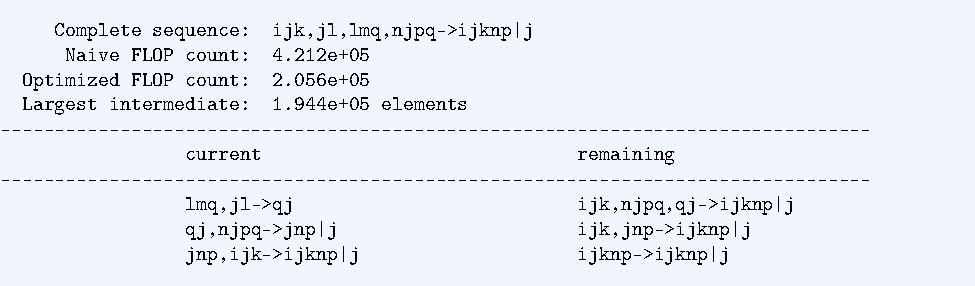
\includegraphics[width=0.98\textwidth]{\fighome/cvoutputfinal.pdf}
\subcaption{\textbf{An optimal sequence of paths.} The code, leveraging \opteinsum with our added support for convolutions, displays the optimal sequence of paths for the \conveinsum string submitted in Figure \ref{fig:cvoutput-a}. We are also presented with information about the naive left-to-right cost vs the cost of taking the suggested path, along with the size/cost of the largest intermediate.}
\label{fig:cvoutput-b}
\end{minipage}
\vspace{-1em}
\caption{\textbf{\conveinsum sample code.} The figure depicts the generation via \numpy of a set of tensors coalesced into one tensor sequence. The sequence is represented as a string and submitted to optimal sequencer of \conveinsum for path analysis. The output of the analysis is presented in Figure \ref{fig:cvoutput-b}.}\label{fig:cvoutput}
\end{figure*}



